\documentclass[a4paper]{article}

\usepackage[english]{babel}
\usepackage[utf8]{inputenc}
\usepackage{amsmath}
\usepackage{amssymb}
\usepackage{bm}
\usepackage{color}
\usepackage[margin=1in]{geometry}
\usepackage{graphicx}
\usepackage[nottoc,numbib]{tocbibind}
\usepackage{float}
\usepackage{multirow}

\renewcommand*{\vec}[1]{\bm{#1}} 		% bold italic version
\renewcommand*{\hat}[1]{\oldhat{\vec{#1}}}
\newcommand\numberthis{\addtocounter{equation}{1}\tag{\theequation}}

\title{On the Terraformation of Mars by Sublimating Trapped CO$_2$ via Bombardment by Non-Planetary Objects}

\author{Team 245}

\date{November 15, 2015}

\begin{document}
  \maketitle

  \begin{abstract}
  In this report we examine one of the early stages in the process of terraforming Mars. From various probes and studies of Mars, we know that CO$_2$ and water-ice are present in solid form at the poles, and extrapolations of known concentrations imply that there is enough CO$_2$ to sufficiently bolster Mars's atmosphere if enough of the ice were to sublimate. We examine estimates for the quantities present and investigate the possibility of releasing enough via impact events to increase Mars's atmospheric pressure past the pressure of the triple point of water with the aim of allowing pure water to exist in stable, liquid form on the surface. We investigate the possible trajectories to send asteroids to Mars, including simple Hohmann transfer-like orbits and more complicated trajectories like those including gravitational assists from Earth or Jupiter, but find that the gravitationally assisted trajectories are impractical or at best inefficient. Finally, we propose a strategy to sublimate the ice while heating the atmosphere by bombarding the surface with a series of nine asteroid impacts followed closely by a single comet impact, as well as calculate a suggested mass for the asteroids and the impulse need to put them on a collision course with Mars.
  \end{abstract}

  \clearpage
  \tableofcontents
  \clearpage
  
  \section{Requirements for Liquid Water on Mars}

	For there to be liquid water on Mars achieved by the sublimation of large amounts of CO$_2$, we found certain requirements that need to be met and certain factors that will cause fluctuations within results.

  \subsection{Liquid Water and Sublimating CO$_2$}
  
  First and foremost is to determine the amount of CO$_2$ that needs to be sublimated into the atmosphere to allow liquid water on Mars. Based on Figure 1, we know that we have to reach a temperature of 273.16 K on Mars and have a consistent atmospheric pressure of at least 611.73 Pa. This would lead us to believe that temperature is the primary focus, however due to the nature of the Martian atmosphere, large variability in pressure and temperature complicate our goal.
  
  \begin{figure}[h]
		\centering
		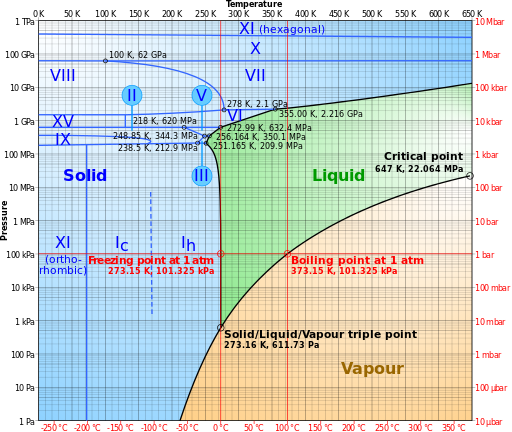
\includegraphics[scale=.5]{Ice_to_water.png}
		\caption{Phase diagram of water \cite{vinayak_vadlamani_if_2015}}
		\label{Figure 1: Phase Diagram}
	\end{figure} \[\]
    
    \begin{figure}[h]
		\centering
		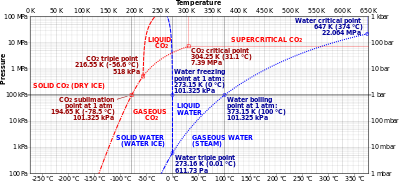
\includegraphics[]{Water_and_CO2.png}
		\caption{Phase diagram of Water and CO$_2$ \cite{vinayak_vadlamani_if_2015}}
		\label{Figure 1: Phase of CO$_2$}
	\end{figure} \[\]
  
  \subsection{Mars's Atmosphere}
  
    Based on empirical information from the Viking 1 mission and the Mars Orbiter Camera, the average surface pressure of Mars at its mean radius is 636 Pa. However, the variability of the seasons on Mars alters the range of the surface pressure at its mean radius from 400 Pa to 870 Pa. \cite{nasa_mars_????} There are certain locations such as the bottom of the Hellas Planitia impact basin, the largest crater on Mars, which reaches an atmospheric pressures of 1155 Pa \cite{wikipedia_climate_2015}. We will be ignoring regions like these because we want a larger region rather than a single creator to allow liquid water when the temperature is above 273K. The average total mass of the Mars atmosphere is $2.5 \times 10^{16}$ kg \cite{nasa_mars_????}. This, like the temperature of Mars, can fluctuate by 25\%.
    
    The mean temperature of Mars is 210 K. The annual temperature range at the Viking 1 Lander site was 184 K to 242 K \cite{nasa_mars_????}. The average temperature based on the Mars Reconnaissance Orbiter found the average temperature near the equator to be to be 195 K to 267 K with record lows and highs of 146 K and 293 K respectively \cite{wikipedia_climate_2015}. Some sources cite that the caps of Mars stay as cold as 100K\cite{wikipedia_climate_2015}.
    
    The reason for these large variations in atmosphere and pressure are due to the seasonal conditions on Mars. These conditions stem from the eccentricity of Mars which is 5 times greater than Mars\cite{wikipedia_mars_2015}. This eccentricity causes the large temperature changes. One key result of these temperature changes is that dry ice will alternate between forming on the north and south poles. This alteration is the primary reason for the changes in pressure on Mars. The pressure changes at the poles are believed to be the reason for the strong winds on Mars that occur during the peak times of accumulation and sublimation of CO$_2$ at the poles.
    
    Based on Mars's atmosphere and temperature, we decided to outline a number of goals that we will be calculating for the energy required and the location of the impacts. With further study and more specific parameters, a more exact calculation for the required energy could be chosen.
    
    \subsection{Source of Greenhouse Gases}
    
    There are a number of sources for CO$_2$ that we took into consideration. The primary sources are the ice caps. The northern ice cap is the smaller of the two and is generally believed to bear a larger portion of water-ice. The reason for the larger portion is due to the northern ice cap often reaching a point above the sublimation of CO$_2$ and lacking some characteristics that lead us to believe that there are larger deposits of CO$_2$ in the southern cap. The southern cap is which larger and colder. Due to geysers there and mapping of the southern pole has led us to find large quantities of CO$_2$.
    
    \subsubsection{Layers on the Mars Ice Caps}
    
    Many sources cite a constant layer of dry ice that is persistent on the southern cap that range in size from .5 meters to 8 meters \cite{david_darling_polar_????}. This would be the easiest layer to sublimate but sadly is small in comparison the required amounts of CO$_2$. Rough estimates of the mass of this layer are $\sim 5 \times 10^{14} kg$. This is no where near the amount that would be needed to effect the atmosphere \cite{stephen_j._mackwell_comparative_2014}.
    
    \subsubsection{Underneath the Mars Ice Caps}
    
    Radar observations by SHARAD have found large deposits of dry ice under the southern cap. These were originally theorized based on the depth of IR signatures. Dry ice is more translucent then water-ice, meaning its depth can be measured by IR radar observations. The largest of the regions is named RFZ$_3$, which in 2011 was observed partially by the Mars Orbital Laser Altimeter\cite{roger_j._phillips_massive_2011}.
    
     \begin{figure}[h]
		\centering
		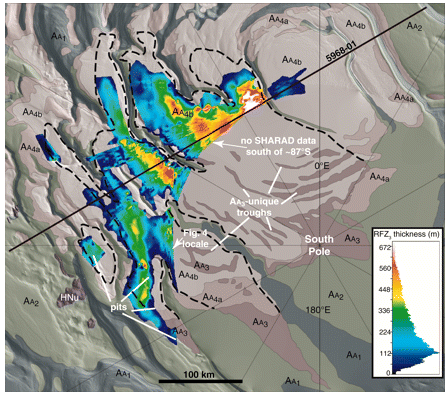
\includegraphics[]{Cool1.PNG}
		\caption{Depth of RFZ$_3$\cite{roger_j._phillips_massive_2011}}
	\end{figure} \[\]
    
    Of the reviewed area, it was estimated that around $9 \times 10^{15}$kg existed. Extrapolation of the entire region estimates that around $2 \times 10^{16}$kg may exist\cite{roger_j._phillips_massive_2011}.
    
     \begin{figure}[h]
		\centering
		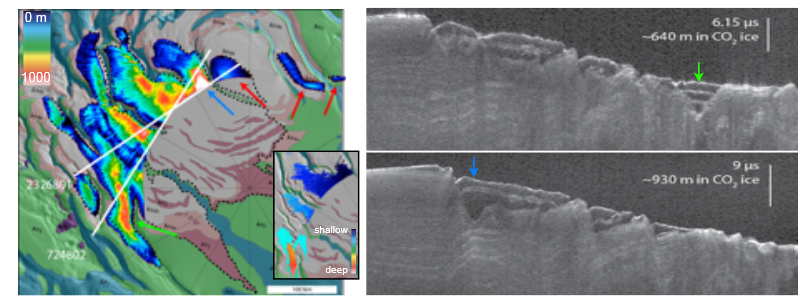
\includegraphics[scale=.5]{Cool2.PNG}
		\caption{Secondary Review of RFZ$_3$ Depth \cite{n._e._putzig_low_2015}}
	\end{figure} \[\]
    
    Later studies found that this region may be closer to $3 \times 10^{16}$kg. The later study even notes that this is a conservative estimate and that the entire region might be larger. This study though is not yet finished, and upon released should be considered\cite{n._e._putzig_low_2015}. These deposits will actually sublimate during the summer at the south pole and are the reason for the geysers on Mars \cite{wikipedia_climate_2015} \cite{roger_j._phillips_massive_2011}. This gives us reason to assume that if we impact the region with asteroids and increase the atmosphere enough to allow liquid water, these deposit would release massive amounts of CO$_2$. These estimates goes as far as more than doubling the total atmosphere of Mars\cite{n._e._putzig_low_2015}.
    
     \subsubsection{Regolith}

  The dust that covers Mars contains a small amount of carbonaceous substances that would be released if Mars were to heat up. However, we found this to be a negligible amount compared to the amount of CO$_2$ that would be needed. Estimates find that the amount of carbon in the Mars soil is around .5\% of the soil density depending on location. \cite{carlton_c._allen_martian_????}
  
  \[m = \dfrac{4}{3} \pi \rho \left({R_M}^3 - \left(R_M - 100 \text{ meters} \right)^3 \right)\]

where $m$ is the carbonaceous substances stored in the first 100 meters of the Mars soil, and $\rho$ being the density of carbon dioxide. This would result in a total mass of about $1 \times 10^{14}$ kg being released.
This mass is negligible compared to the atmospheric mass of $2.5 \times 10^{16}$ kg since our goal is at least changing atmospheric conditions by 10\%. Consequently, we ignored the the Mars regolith as a source although future research could take this into account.

    \subsection{Energy Required}
    
    To approximate the energy required for the sublimation of CO$_2$ on Mars we used:
    
    \[ E = m \cdot C \cdot \Delta T\]
    
    Where $E$ is the energy required to change the temperature by $\Delta T$ of a the mass $m$ with a specific heat of $C$. Depending on the whether the CO$_2$ is pressurized or already in the atmosphere,  we could be using either C$_p$ or C$_v$ for C, the specific heat when under a constant pressure or under a constant volume respectively. However for simplification, we will just use the average of the two specific heats of .75 kJ/kg K.
    
    \begin{table}[H]
		\centering
		\caption{Carbon Dioxide Specific Heat \cite{flsmidth_gases_????}}
		\begin{tabular}{|c|c|}
		\hline
		\multicolumn{2}{|c|}{Specific Heat Capacity} \\ \hline
		$C_p  (kJ/kg\ K)$                    & $C_v (kJ/kg\ K)$                   \\ \hline
		.844                  & .655                 \\ \hline
		\end{tabular}
	\end{table}
    
    The reasons for the below temperatures is that an increase of 21K would bring the average minimum at the Viking 1 Lander Site to the needed 273K. The reason for 63K is that it is the mean temperature NASA lists for Mars. A change of 89K would bring the minimum mean temperature of Mars to the required level. 170K would bring the entire southern pole to a level that would allow liquid water (Note: This is to allow liquid water there, it would take larger amounts of energy to turn all of it into water). The masses of CO$_2$ comes from the amount already in the atmosphere, the amount that is known to be stored in the southern cap and the amount that is extrapolated based on observations to be stored in the southern cap.

\begin{table}[H]
\centering
\caption{Energy Required for $2.5 \times 10^{16}$kg of CO$_2$}
\begin{tabular}{|c|c|c|c|c|}
\hline
    			  & \multicolumn{4}{c|}{Atmospheric Temperature Change (Kelvin)} \\ \cline{2-5} 
   				  & 170            & 89            & 63           & 31           \\ \hline
Energy Required (kJ)&   $3.185 \times 10^{18}$             &      $1.668 \times 10^{18}$          &   $1.18 \times 10^{18}$            &   $5.809  \times 10^{17}$          \\ \hline
\end{tabular}
\end{table}

\begin{table}[H]
\centering
\caption{Energy Required for $3.75 \times 10^{16} $kg of CO$_2$}
\begin{tabular}{|c|c|c|c|c|}
\hline
    			  & \multicolumn{4}{c|}{Atmospheric Temperature Change (Kelvin)} \\ \cline{2-5} 
   				  & 170            & 89            & 63           & 31           \\ \hline
Energy Required (kJ)&   $4. 778\times 10^{18}$             &      $1.668 \times 10^{18}$          &   $1.771 \times 10^{18}$            &   $8.713  \times 10^{17}$          \\ \hline
\end{tabular}
\end{table}

\begin{table}[H]
\centering
\caption{Energy Required for $5 \times 10^{16}$kg of CO$_2$}
\label{ENERGY}
\begin{tabular}{|c|c|c|c|c|}
\hline
    			  & \multicolumn{4}{c|}{Atmospheric Temperature Change (Kelvin)} \\ \cline{2-5} 
   				  & 170            & 89            & 63           & 31           \\ \hline
Energy Required (kJ)&   $6.371\times 10^{18}$             &      $3.335\times 10^{18}$          &   $2.361\times 10^{18}$            &   $1.162  \times 10^{18}$          \\ \hline
\end{tabular}
\end{table}

  \subsection{Asteroids}

  An important factor when considering what asteroid to use is foremost its size, composition and location.

  \subsubsection{Composition}

  There is a defined system of asteroid classifications that defines the asteroids into their compositions. These compositions reach beyond what we are interested in, and instead we will simply focus on two of the most common types that we will consider using. There are two typical compositions that we should consider. First, there are Iron Asteroids which are more dense and more plentiful within the asteroid belt. The composition of these iron asteroids are generally 91\% iron and 9\% nickel along with other metals \cite{charles_choi_asteroids:_2014}. Second, there are sedimentary asteroids that are composed of lighter elements. A typical composition of a sedimantary asteroid would be 36\% oxygen, 26\% iron, 18\% percent silicon, 14\% magnesium and other elements \cite{charles_choi_asteroids:_2014}.

  The reason we are interested in these two general compositions is that they will have different properties during an impact event. We estimate the Iron asteroids to have a density around 8000 kg/m$^3$, which means they would not break up on entry and would be better suited for deeper, more penetrating impacts. An estimation for sedimentary asteroid density can be found around 3000 kg/m$^3$. \cite{gareth_s._collins_earth_2005} These lighter sedimentary asteroids are more likely to breakup and become an airburst impact. Airburst impacts, though not as deep, would be capable of impacting a much wider area.
  
  \subsubsection{Simulating Impacts}
  We used the simulation software called ImpactEarth! \cite{itap_for_purdue_university_impact_????} for a rough approximation of the impact and destructive capabilities of asteroids. In our simulations, we found that breaking the layer of water-ice on the south pole would be fairly easy and would only require a few kilometer large asteroid. Otherwise we are interested in looking at the impact effecting the largest possible area. This simulation assumes the impact is happening on Earth, however the documentation included with it could allow a simulation to be built that would be focused on Mars. Further research and development of a simulation would have to take into account the changing atmosphere of Mars during the impacts\cite{gareth_s._collins_earth_2005}. 

  \subsubsection{Asteroid Location}

  For this paper, we have decided to focus only on asteroids that are within the core asteroid belt. This allows for a large variety of asteroids, with over .7 to 1.7 million asteroids existing in this region including some with a 1 km diameter or greater. This abundance of asteroids also has a large radial distribution, stretching from 2.1 AU to 3.3 AU. There are some exceptions to an even distribution, notably that asteroids are not found at the Kirkwood gaps, the points that due to orbital resonance with Jupiter will destabilize any orbits. \cite{edward_f._tedesco_infrared_2002} In a circular orbit, the velocity can be easily found by Kepler's third law:
  
  \[P_1 = \sqrt{{P_2}^2 \left(\dfrac{a_1}{a_2}\right)^{\!\!3}}\]
  \[v = \dfrac{2\pi a_1}{P_1} = 2\pi \sqrt{\dfrac{{a_2}^3}{{P_2}^2 a_1}}\]
  We will primarily consider three different initial radial positions of asteroids in order to get a good range of parameters.
  \begin{table}[ht]
  \centering
  \caption{choices of asteroids}
  \label{}
  \begin{tabular}{c|c|c}
  asteroid & semi-major axis & velocity \\ \hline
  inner      & 2.2 AU & 20.1 km/s \\ \hline
  central      & 2.7 AU & 18.1 km/s \\ \hline
  outer      & 3.2 AU & 16.7 km/s
  \end{tabular}
  \end{table}

  \subsubsection{Limitations of Comets}
  We considered using a fleet of ten comets instead of the ten asteroids. The orbital parameters of many asteroids are known, but orbital parameters are only known for relatively few comets. Additionally, comets have lower densities because they are composed of loosely packed rock, ice, and other materials, rather than solid, rock, or metal. They are also much more widely spread out and would require several radically different missions to redirect them. Whereas with asteroids, we can pluck them all out of the asteroid belt. Similarly, timing the impacts of comets to all be within the same time would be extremely difficult due to their very wide range of parameters. Thus, we limit ourselves to only one comet and would match our asteroids' timing to it.

	\section{Orbital Mechanics}
	\subsection{Hohmann Transfer-Like Path to Mars}
	The simplest method of transferring an asteroid to an orbit that will intersect Mars is by the use of a single velocity boost parallel to its direction of motion. This would effectively be the same as the first of the two stages of a Hohmann transfer, assuming that Mars's orbit and the orbits of asteroids in the asteroid belt are approximately circular. Although they have nonzero eccentricity and the eccentricity of Mars's orbit plays an important role in its weather cycles, we will neglect the eccentricity for simplicity. Then the semi-major axis of the transfer orbit is
	\[a = \dfrac{1}{2} \left(a_M + aA\right)\]
	where $a_A$ is the semi-major axis (and radius, since the orbit is circular) of the orbits in the asteroid belt, and $a_M$ that of Mars.
	The energy of this orbit is
	\[E = -\dfrac{G M m}{2a} = -\dfrac{m \mu}{a_M + a_A}\]
	and we define $\mu \equiv G M$ as the standard gravitational parameter. The energy of the asteroid's original orbit is
	\[E_0 = -\dfrac{m \mu}{2 a_A}\]
	and the difference will tell us how much energy we need to provide. This difference is equal to the difference in kinetic energies as the potential energies are the same at the moment of boosting.
	\begin{align*}
	\Delta E &= E - E_0 = \Delta T \\
	&= \dfrac{1}{2} m \left(v_A + \Delta v\right)^2 - \dfrac{1}{2} m {v_A}^2
	\end{align*}
	To find the velocity boost needed, we use the energy at aphelion.
	\begin{align*}
	E &= -\dfrac{m \mu}{a_M + a_A} = \dfrac{1}{2} m {v_1}^2 - \dfrac{m \mu}{a_A} \\
	v_1 &= \sqrt{\dfrac{2 \mu}{a_A} - \dfrac{2 \mu}{a_M + a_A}} \numberthis \label{totvel} \\
	&= \sqrt{2\mu \left(\dfrac{a_M}{a_A \left(a_M + a_A\right)}\right)}
	\intertext{Taking the initial velocity of the asteroid to be $v_A = \sqrt{\mu / a_A}$,}
	v_1 &= v_A \sqrt{\dfrac{2 a_M}{a_M + a_A}}
	\intertext{The boost $\Delta v$ that we must provide is the difference.}
	\Delta v &= v_1 - v_A = v_A \left[\sqrt{\dfrac{2a_M}{a_M + a_A}} - 1\right] \numberthis
	\end{align*}
	
	\begin{figure}[ht]
		\centering
		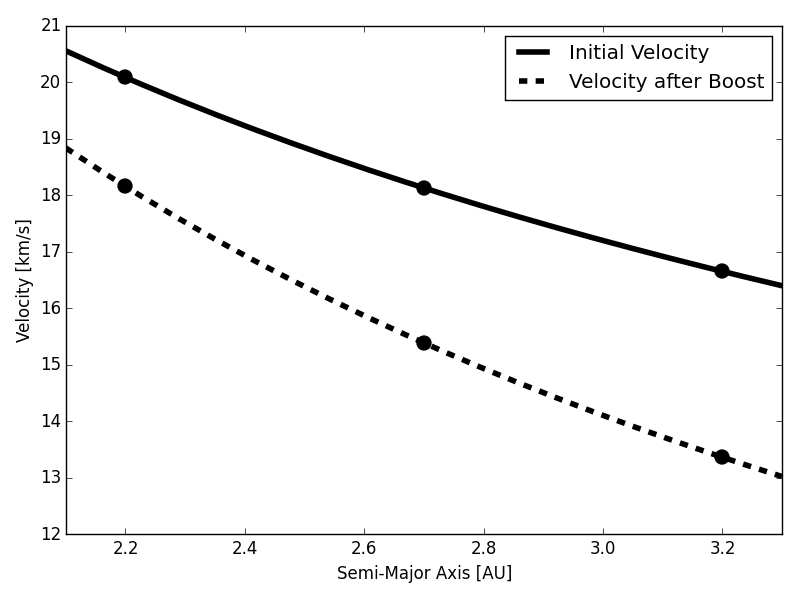
\includegraphics[scale=0.5]{velocity.png}
		\caption{Velocity vs. Initial Semi-Major Axis}
		\label{fig:vel1}
	\end{figure} \[\]
	
	Figure \ref{fig:vel1} shows the velocities for various distances from the Sun. For our sample asteroids:
	
	\begin{center}
		delta-$v$ for simple Mars impact
		
		\begin{tabular}{c|c}
			asteroid & $\Delta v$ \\ \hline
			inner      & -1.9 km/s \\ \hline
			central      & -2.74 km/s \\ \hline
			outer      & -3.3 km/s
		\end{tabular}
	\end{center}
	
	These values are negative because we need to slow the asteroids down with respect to the center of mass of the solar system in order to transfer from the orbit of the asteroid belt to the smaller orbit of Mars. The velocity of the asteroid at impact with Mars can be found by conservation of angular momentum.
	\begin{align*}
	\vec{L}_1 &= \vec{L}_2 \\
	\vec{r}_A \times \vec{p}_1 &= \vec{r}_M \times \vec{p}_2
	\end{align*}
	At aphelion and perihelion, $\vec{r} \perp \vec{p}$, so the cross products simplify. The mass is constant, so
	\begin{align*}
	v_2 &= v_1 \dfrac{a_A}{a_M} = \left(v_A + \Delta v\right) \dfrac{a_A}{a_M}
	\end{align*}
	Note that we take $a_M = 1.52$ AU. When it reaches Mars via this orbit, their velocities will be parallel. The relative velocity as the asteroid approaches is $v_2 - v_M$, and we take $v_M = 24.1$ km/s. Generally, it would be
	\[v_2 - v_M \cos\phi \numberthis \label{gen1}\]
	where $\phi$ is the angle between the velocity of the asteroid and the velocity of Mars, but here $\phi \simeq 0$. The velocity that the asteroid would impact Mars with, assuming the atmosphere is initially thin enough to not significantly limit the speed, is this approach velocity plus the escape velocity of Mars. Escape velocity is
	\begin{align*}
	v_e &= \sqrt{\dfrac{2G M_M}{r_M}} = 5.0 \text{ km/s} \\
	v &= \left(v_A + \Delta v\right) \dfrac{a_A}{a_M} + v_e - v_M \\
	v &= v_A \dfrac{a_A}{a_M} \sqrt{\dfrac{2a_M}{a_M + a_A}} + v_e - v_M \numberthis \label{impact}
	\end{align*}
	
	\begin{figure}[ht]
		\centering
		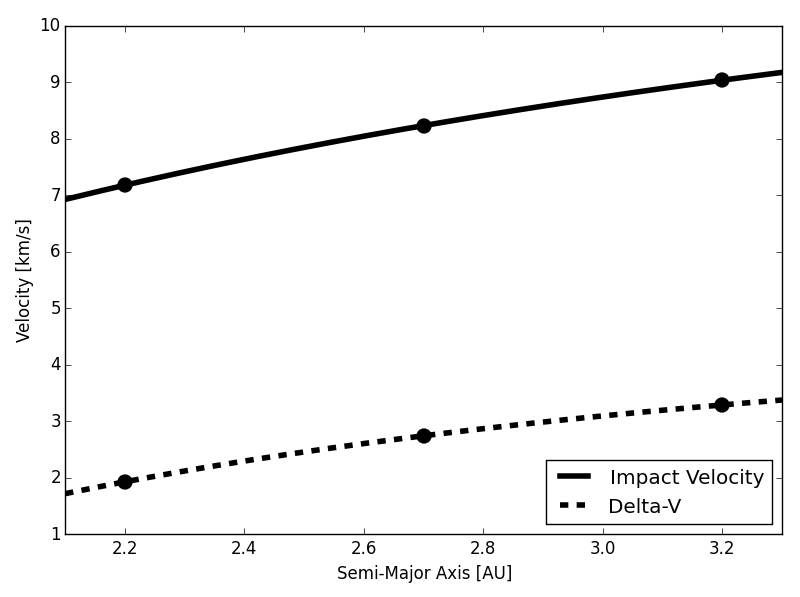
\includegraphics[scale=0.5]{velocity2.png}
		\caption{Impact Velocity vs. Initial Semi-Major Axis}
		\label{fig:vel2}
	\end{figure} \[\]
	
	\begin{center}
		impact velocity for sample asteroids
		
		\begin{tabular}{c|c}
			asteroid & impact velocity \\ \hline
			inner      & 7.2 km/s \\ \hline
			central      & 8.2 km/s \\ \hline
			outer      & 9.1 km/s
		\end{tabular}
	\end{center}
    
    \subsection{Mass and Impulse}
    From the simulations using the ImpactEarth! utility and given the estimated sizes of the ice deposits, we found that a diameter of 100 meters for each of the nine asteroids will yield a satisfactory quantity of CO$_2$ exposed. We can now see what their kinetic energy will be at impact and also the impulse we would need to provide them to send them on their paths. Each one's mass is
    \begin{align*}
    m &= \dfrac{4}{3} \pi r^3 \rho \\
    m &\sim 1.0 \times 10^9 \text{ kg}
    \end{align*}
    
	\begin{center}
		energy and impulse for the asteroids
		
		\begin{tabular}{c|c|c}
			asteroid & kinetic energy [J] & impulse needed [kg $\cdot$ m/s] \\ \hline
			inner      & $2.6 \times 10^{16}$ J & $7.2 \times 10^{12}$ \\ \hline
			central      & $3.4 \times 10^{16}$ J & $8.2 \times 10^{12}$ \\ \hline
			outer      & $4.1 \times 10^{16}$ J & $9.1 \times 10^{12}$
		\end{tabular}
	\end{center}
    
	\subsection{Asteroid Trajectory Efficiency}
	
	Figure \ref{fig:vel2} shows the velocity at impact for various initial distances from the Sun. Of particular interest is the ratio of the impact velocity to the delta-v imparted. Higher values of this ratio correspond to higher efficiency: getting more impact velocity per unit impulse. This ratio is shown in Figure \ref{fig:vel3}.
	
	\begin{figure}[ht]
		\centering
		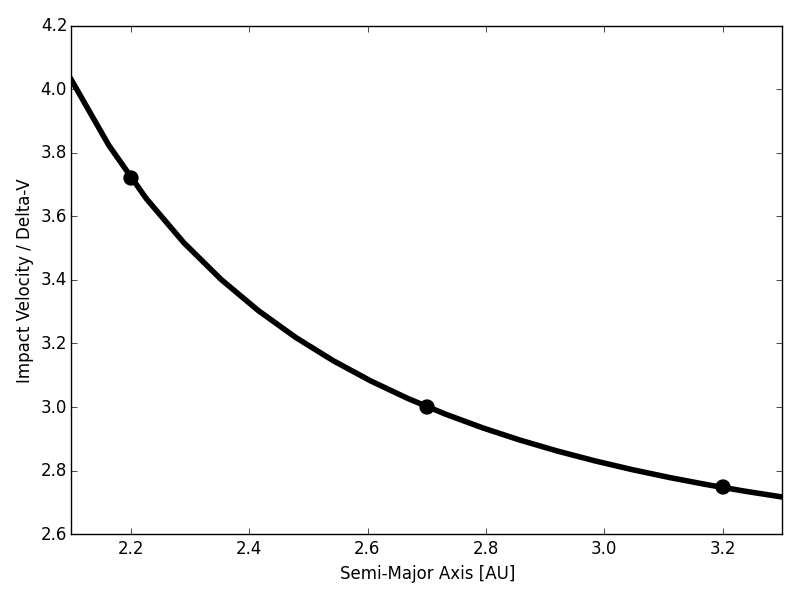
\includegraphics[scale=0.5]{ratio.png}
		\caption{Delta-V Efficiency Ratio}
		\label{fig:vel3}
	\end{figure} \[\]
	
	Providing a larger delta-$v$, still parallel to the asteroid's initial velocity, would result in a direct boost to the impact velocity greater than the additional delta-$v$. That is, if we add a small additional delta-$v$ to eqn. \eqref{impact}, the impact velocity would be
	\begin{align*}
	v &> v_A \dfrac{a_A}{a_M} \sqrt{\dfrac{2a_M}{a_M + a_A}} + v_e - v_M
	\intertext{because the asteroid's velocity and Mars' will no longer be parallel (the asteroid would now actually cross Mars' orbit rather than just touch it, if Mars were not in the way), meaning that from eqn. \eqref{gen1}, we will have}
	v &\simeq v_A \dfrac{a_A}{a_M} \sqrt{\dfrac{2a_M}{a_M + a_A}} + v_e - v_M \cos\phi
	\end{align*}
	where $\phi > 0$. This equation is approximate because the altered velocity will mean that the first term is not quite exact, but is close in the regime that the extra velocity is small. Finding this angle $\phi$ as a function of the initial delta-$v$ and developing a generalized impact velocity relation would be a good area to explore in the future. In the limit that the initial delta-$v$ approaches the asteroid's velocity, directed oppositely, $\phi \rightarrow \pi/2$ and we would be hitting Mars perpendicularly.
	
	\subsection{Other Paths to Mars}
	\subsubsection{Motivation}
	Seeing that the fact that the asteroids and Mars are traveling in approximately parallel directions during the approach due to their common prograde orbits, and that this means we are fighting Mars' orbital velocity of 24.1 km/s, we decided to investigate possible ways around this. We considered utilizing a gravitational assist from a planet---either Jupiter or Earth---to change the asteroid's motion from prograde to retrograde. This would ideally allow the asteroid to hit Mars head-on instead of catching up to it.
    As an analogy, it would be like a head-on collision between two cars each going 100 km/h rather than a rear-end collision between a car going 100 km/h and a car going 105 km/h. The head-on collision would have a much higher energy for the same asteroid velocity. This means that we might be able to select asteroids of lower mass, giving them the same velocity, expending less impulse, but retaining or even increasing the impact energy.
	\subsubsection{Analysis}
	Near the planet, we assume the gravitational effect of the planet is much stronger than that of the Sun, and thus only consider the planet. The asteroid would take a hyperbolic orbit around the assisting planet. Let $b$ be the impact parameter, $v_0$ the relative velocity that the asteroid approaches the planet with. By conservation of energy starting from far away from the planet,
	\begin{align*}
	\dfrac{1}{2} m {v_0}^2 &= \dfrac{1}{2} m v^2 - \dfrac{m \mu}{r}
	\intertext{with $\mu$ now referencing the planet's mass rather than the Sun's.}
	v &= \sqrt{{v_0}^2 + \dfrac{2\mu}{r}}
	\intertext{Also, the closest approach is}
	\dfrac{1}{2} m {v_0}^2 &= \dfrac{1}{2} m \dfrac{{v_0}^2 b^2}{r^2} - \dfrac{m \mu}{r} \\
	0 &= {v_0}^2 r^2 + 2\mu r - {v_0}^2 b^2 \\
	\intertext{Throwing away the negative solution,}
	r &= \dfrac{-\mu + \sqrt{\mu^2 + {v_0}^4 b^2}}{{v_0}^2}
	\end{align*}
	By conservation of momentum, assuming that the path has not changed much by the time the asteroid gets to the planet
	\begin{align*}
	m v_0 b \simeq m v r
	\intertext{where $v$ and $r$ correspond to the velocity and orbit radius at closest approach.}
	b &= \dfrac{v r}{v_0} \\
	b &= \sqrt{r^2 + \dfrac{2\mu r}{{v_0}^2}}
	\end{align*}
	Let us define the total deflection of the asteroid as $2 \theta$. Then, using the formula for hyperbola excess velocity,
	\begin{align*}
	v_0 &= \sqrt{\dfrac{\mu}{-a}}
	\intertext{where $a$ is the (negative) semi-major axis of the hyperbolic orbit.}
	a &= -\dfrac{\mu}{{v_0}^2} \\
	\sin\theta &= \dfrac{b}{r + a}
	\end{align*}
	\begin{align*}
	\theta &= \arcsin\left(b \left(\dfrac{\mu}{{v_0}^2} + \dfrac{-\mu + \sqrt{\mu^2 + {v_0}^4 b^2}}{{v_0}^2}\right)^{-1}\right) \\
	&= \arcsin\left(\left(\sqrt{\dfrac{\mu^2}{{v_0}^4 b^2}} + 1\right)^{-1}\right)
	\end{align*}
	If we pick a safe distance of closest approach $r_s$ large enough to not risk collision with the planet (somewhere in the range of $1.1 r$ to $1.5 r$) we can find the impact parameter
	\begin{align*}
	b &= \sqrt{{r_s}^2 + \dfrac{2\mu r_s}{{v_0}^2}}
	\end{align*}
	and the deflection angle. As we found out, the deflection will unfortunately not be sufficient to send the asteroid in a retrograde orbit (at least, for most reasonable values of delta-$v$). While reversed relative to the planet, the overall motion is still in the prograde direction since the maneuver costs the asteroid speed relative to the Sun. We have not done an exhaustive search of the trajectories, however; there may be a handful of ways to rescue this strategy but this will require further analysis.
	
	\subsection{The Final Blow --- Retrograde Comet}
	\subsubsection{Motivation}
	Our goal is to sublimate enough of the frozen CO$_2$ to create an atmosphere with enough pressure to support liquid water. As discussed earlier, most of the CO$_2$ is clumped at the poles. We suggest that several of the impactors be directed at the southern pole, where the largest concentration of CO$_2$ is believed to be. A series of impact events will serve to break through the layer of water ice covering the majority of the CO$_2$, as well as dispersing much of their energy as heat to the atmosphere. Since very precise placement of the impacts would be very difficult given just an initial push, we propose that nine of the ten impactors be asteroids from the inner edge of the asteroid belt, while the tenth and final impactor will be a comet traveling in the retrograde direction at much higher relative velocity than the asteroids. This strategy would serve to break up the ice layers and expose them to the atmosphere, while heating the atmosphere, leaving large quantities of the underground frozen CO$_2$ exposed and vulnerable to a single higher-energy impact event from the comet, allowing more uniform distribution of energy and ultimately more sublimation.
	
	Additionally, one more advantage of using a comet is that if we provide the push when it is at its aphelion, the impulse necessary would be very small compared to even that of an asteroid, because the comet's velocity is very small at aphelion. The obvious disadvantage is that the period of a comet's orbit is long, and its aphelion is far away. Thus, it would be a difficult and time-consuming process to be able to boost the comet at aphelion and wait for it to reach Mars. Since the asteroids from the belt would take much less time to reach Mars, we suggest beginning the mission to the comet much earlier than the missions to the asteroids. Then, time the impulses so that the asteroids will arrive within a small span of time and the comet will arrive soon after.
	\subsubsection{Analysis}
	Let us discuss a fictional comet designated Temoc with (hopefully) representative parameters and properties (for familiarity we base its details off of Halley's Comet, except the mass which we'll make smaller by a factor of one hundred, representing a rather small comet). It has a semi-major axis of 17.8 AU, a distance at perihelion $r_p$ of 0.6 AU, and a mass of $2 \times 10^{12}$ kg. The aphelion distance is $r_a = 2a - r_p = 35$ AU. For simplicity, the inclination of the orbit is assumed to be zero (more correctly, the inclination is $180^\circ$, because it is in retrograde motion). From the vis-viva equation
	\begin{align*}
	v &= \sqrt{\mu \left(\dfrac{2}{r} - \dfrac{1}{a}\right)} \\
	v &= \begin{cases}
	53.9 \text{ km/s} & \text{at perihelion} \\
	0.920 \text{ km/s} & \text{at aphelion}
	\end{cases}
	\end{align*}
	Now we calculate the impulse we would need to give Temoc in order to achieve a head-on collision with Mars via a Hohmann transfer-like path and the resulting impact velocity. The total velocity it needs at aphelion is given by eqn. \eqref{totvel}:
	\begin{align*}
	v_1 &= \sqrt{\dfrac{2 \mu}{r_a} - \dfrac{2 \mu}{r_a + a_M}} \\
	&= 1.453 \text{ km/s}
	\end{align*}
	and so the boost we must give is
	\begin{align*}
	\Delta v &= v_1 - v_a = \sqrt{\dfrac{2 \mu}{r_a} - \dfrac{2 \mu}{r_a + a_M}} - \sqrt{\mu \left(\dfrac{2}{r_a} - \dfrac{1}{a}\right)} \\
	&= 1.453 \text{ km/s} - 0.920 \text{ km/s} \\
	&= 0.533 \text{ km/s}
	\end{align*}
	This delta-$v$ is several times less than what was required for the asteroids. The impulse required is
	\begin{align*}
	\Delta p &= m \Delta v \\
	&= 1.066 \times 10^{15} \text{ kg $\cdot$ m/s}
	\end{align*}
	The velocity of approach to Mars is
	\begin{align*}
	v_2 &= v_1 \dfrac{r_a}{a_M}
	\intertext{Now we add Mars' orbital velocity to find the relative velocity rather than subtract it as before, since the comet is traveling in a retrograde direction and the collision is head-on. The relative velocity is}
	v_2 + v_M &= v_1 \dfrac{r_a}{a_M} + v_M
	\intertext{and the impact velocity is found by adding the escape velocity of Mars. The final impact velocity is}
	v &= v_2 + v_M + v_e \\
	v &= 62.56 \text{ km/s}
	\end{align*}
	The impact energy is, from $T = \dfrac{1}{2} m v^2$,
	\begin{align*}
	T &= 3.9138 \times 10^{18} \text{ kJ}
	\end{align*}
    Referencing table \ref{ENERGY}, we see that we are within a small factor of the calculated necessary energies. Despite small errors such as that not all of the kinetic energy will be dispersed as heat, or the leftover energy from the asteroids, this comet should raise the temperature of the atmosphere by an amount very close to what we need. From $E = m \cdot C \cdot \Delta T$, the temperature change will be approximately 100 K.
    
    
    \section{Conclusion}
    Given the promising but limited information we have so far about the ice at Mars' polar caps, it should be possible to release enough gas to create an atmospheric pressure high enough to permit liquid water. We utilize nine asteroid impacts aimed at the southern polar cap to attempt to break apart the ice and rock, followed by a comet impact to sublimate the ice and warm the atmosphere. The asteroids would have masses each around $1 \times 10^9$ kg and would need impulses of between $7.2 \times 10^{12}$ kg $\cdot$ m/s and $9.1 \times 10^{12}$ kg $\cdot$ m/s. The comet would have a mass of about 1\% that of Halley's comet and would need an impulse of approximately $1.1 \times 10^{15}$ kg $\cdot$ m/s, and a mass of $2 \times 10^{12}$ kg.
    
Our calculations have shown the size and the impulse each impactor needs in order to sufficiently intersect with Mars and consequently warm the atmosphere. These are the early stages of terraforming Mars through heating the planet to a climate that is suitable enough for stable liquid water utilizing a series of impacts. 
    \clearpage
	\appendix
	\section{Appendix}	
	\subsection{Mars}
    Included is data on Mars \cite{nasa_mars_????}.
	\begin{itemize}
		\item[$\cdot$] Semi-major axis: $227.92 \times 10^5$ km
		\item[$\cdot$] Mean radius: $3389.5$ km
		\item[$\cdot$] Mass: $6.4174 \times 10^{23}$ km
		\item[$\cdot$] Surface gravity: $3.71$ m/s$^2$
		\item[$\cdot$] Surface density: $\sim 0.020$ kg/m$^3$
		\item[$\cdot$] Composition
		\subitem- (CO2) - 95.32\%
		\subitem- Nitrogen (N2) - 2.7\%
		\subitem- Argon (Ar) - 1.6\%
		\subitem- Oxygen (O2) - 0.13\%
		\subitem- Carbon Monoxide (CO) - 0.08\%
		\item[$\cdot$] Average temperature range: 184 K to 242 K based on Viking 1 Lander
	\end{itemize}
	
	\subsection{Misc.}
	\begin{itemize}
		\item[$\cdot$] Density of CO$_2$ as a solid = $1.98$ kg/m$^3$ \cite{wolfram_alpha_llc_wolframalpha_2015}
	\end{itemize}
	
  \clearpage
  \bibliographystyle{ieeetr}
  \bibliography{Zotero}
\end{document}